%! suppress = FileNotFound
\documentclass[conference]{IEEEtran}
\IEEEoverridecommandlockouts


\usepackage{cite}
\usepackage{csquotes}
\usepackage{graphicx}
\usepackage{textcomp}
\usepackage{xcolor}
\usepackage{hyperref}

%! suppress = DiscouragedUseOfDef
\def\BibTeX{{%! suppress = PrimitiveStyle
\rm B\kern-.05em{%! suppress = PrimitiveStyle
\sc i\kern-.025em b}\kern-.08em
T\kern-.1667em\lower.7ex\hbox{E}\kern-.125emX}}

\begin{document}
\title{'Some title'}

\author{
	\IEEEauthorblockN{1
		\textsuperscript{st} Bachmann Lucius
	}
	\IEEEauthorblockA{
		\textit{Department of Informatics} \\
		\textit{University of Zurich}\\
		Zurich, Switzerland \\
		lucius.bachmann@gmx.ch
	}
}

\maketitle

\begin{abstract}
	Cloud computing is pervasive in the software industry.
With the advancement of web technology it is now possible to fulfill most of the computing needs as a service
in the cloud.
The services offering cloud services are also using other cloud services to perform their computing.
The development effort to develop and deploy an application to the cloud becomes less every year.
This also allows to use testing tools in the cloud to speed up the development and reduce cost for the development.
The following paragraphs will show how small to medium sized applications can leverage the cloud to test their application.

\end{abstract}

\begin{IEEEkeywords}
	component, formatting, style, styling, insert
\end{IEEEkeywords}

\section{Introduction}

\subsection{Technological terms}

\subsubsection{OCI containers and docker}

The Open Container Initiative (OCI) is a project to create standards around containers\cite{oci-webiste}.
Containers are a way to package (image spec), distribute (distribution spec) and run (runtime spec) an application
which may consist of binaries or a script with its interpreter.
The application can be shipped with all it's dependencies that the runtime does not need to adhere to any
requirements except for the runtime spec.
But a container is not a virtual machine with all its drawbacks, the kernel of a container is shared with the host system.
Thus the image of a container can be smaller and running the container needs almost always less resources than running the same application
in virtual machine.
Docker Inc\. offers one implementation of the OCI specifications with a build tool for OCI images (buildkit), a runtime (containerd)
and a cli (docker-cli) to interact with the build tool and the runtime\cite{docker-container-runtime-website}.

\subsubsection{Kubernetes}

Kubernetes is a tool developed and open sourced by Google to manage and orchestrate multiple containers.
It allows to configure which containers should run, under which port which container is accessible,
how the containers can interact with each other, under which conditions a container is considered healthy and it also allows
to inject configuration files, environment variables and secrets into the container.
With the configuration the user describes the state in which the cluster should be, and kubernetes then performs the
operations like starting a container, configuring the network or injecting configuration to reach this state.
If a container crashes and the cluster deviates from the configured state, kubernetes can automatically detect that
the state deviated and then tries to restore the desired state by e.g.\ restarting a container.
Kubernetes can also be used on multiple nodes, where one main node can deploy the containers to many child nodes
and thus provide an easy way for horizontal scaling.

\subsubsection{Helm}

Helm is package manager for kubernetes\cite{helm-website}.
A collection of kubernetes configuration files can be packaged together and published as helm chart on a repository
like artifacthub.io\cite{artifacthub-io}.
Helm also offers the possibility to use templates for your kubernetes configuration files, that the helm chart
can be adapted when it's deployed to a kubernetes cluster.

\subsubsection{Github Actions}

Github Actions is a CI/CD service offered by Github\cite{github-actions-website}.
It allows to configure workflows with yaml which integrate well with the version control, review
and issue tracking system of github itself.
A workflow consists of trigger events like a git push to a branch, a pull request, a manual workflow dispatch or
other triggers and jobs.
In each job the different steps can be defined to build, test or deploy a service.
An example for such a workflow can be found at the following link: \href{https://github.com/ecamp/ecamp3/blob/7a1cf92e3eee27b0b942fcd87bd8ce5c221089b7/.github/workflows/reusable-build-and-push.yml}{ecamp3/reusable-build-and-push.yml}.
For each job a virtual machine is provisioned in which this job is executed\cite{github-actions-about-runner}.

\section{eCamp Version 3}

eCamp is a web application to help with organising camps for youth organisations like the
scouts, YMCA (Young Men Christian Organisation)\cite{ymca-website} and YWCA or the Jubla.
It allows to collaboratively schedule the activities during the camp and to plan them in detail
according to the regulations of the swiss federal support program for sport activities (Y+S) with young people\cite{J+S-Website,ecamp3-website}.
eCamp version 2 is live since at least 2010\cite{ecamp2-first-commit} and was already used to plan a lot of camps.
The new version 3 is in development since 5 years\cite{ecamp3-website} with the goal to separate frontend and backend and
to leverage known, active and newer frameworks for frontend and backend for their bug and security fixes and
their new features to improve the usability, accessibility and maintainability of the application.

\subsubsection{Technology stack}

\subsubsection{Architecture}

The application uses 5 components depicted in figure\ref{fig:ecamp3-architecture}.
The frontend is a Vue application bundled with vite and served by a nginx web server.
The api is a PHP application using the API Platform framework which also served by a web server.
The print service is a nuxt application which lets the browserless container visit itself to render a printable
html of an activity, schedule or a whole camp and convert it to a pdf, which is then served back to the frontend.

\begin{figure}[h!]
	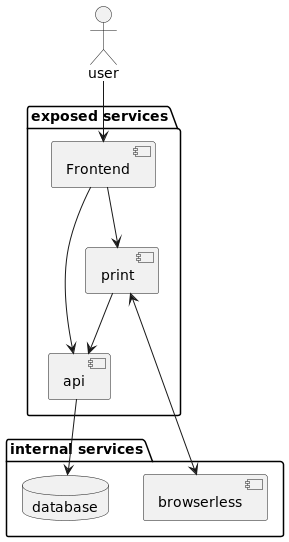
\includegraphics[height=\columnwidth]{sections/assets/ecamp3-architecture}
	\caption{eCamp V3 Architecture}
	\label{fig:ecamp3-architecture}
\end{figure}

\subsubsection{Deployment}

The application is currently deployed to a kubernetes cluster of DigitalOcean.
As database a managed postgres instance is used which already includes scalability and backups for 5 days.
To separate the stages 3 clusters for development, staging and production are in use.
For all self developed services the respective applications are packaged with docker in an OCI image and then
pushed to docker hub with github actions\cite{ecamp3-reusable-build-and-push}.
Then these images are deployed with a helm chart to the respective kubernetes cluster\cite{ecamp3-reusable-dev-deployment, ecamp3-deployment-stage-prod}.

\section{Related work}

\section{Background}

\section{Method}

\section{Experiment}

\section{Conclusion}

\bibliographystyle{IEEEtran}
\bibliography{main}

\date{\today}



\newpage
%
\end{document}